\newpage
\subsection{Caso d'uso UC9: Gestione dei questionari}
\label{UC9}
\begin{figure}[h]
	\centering
	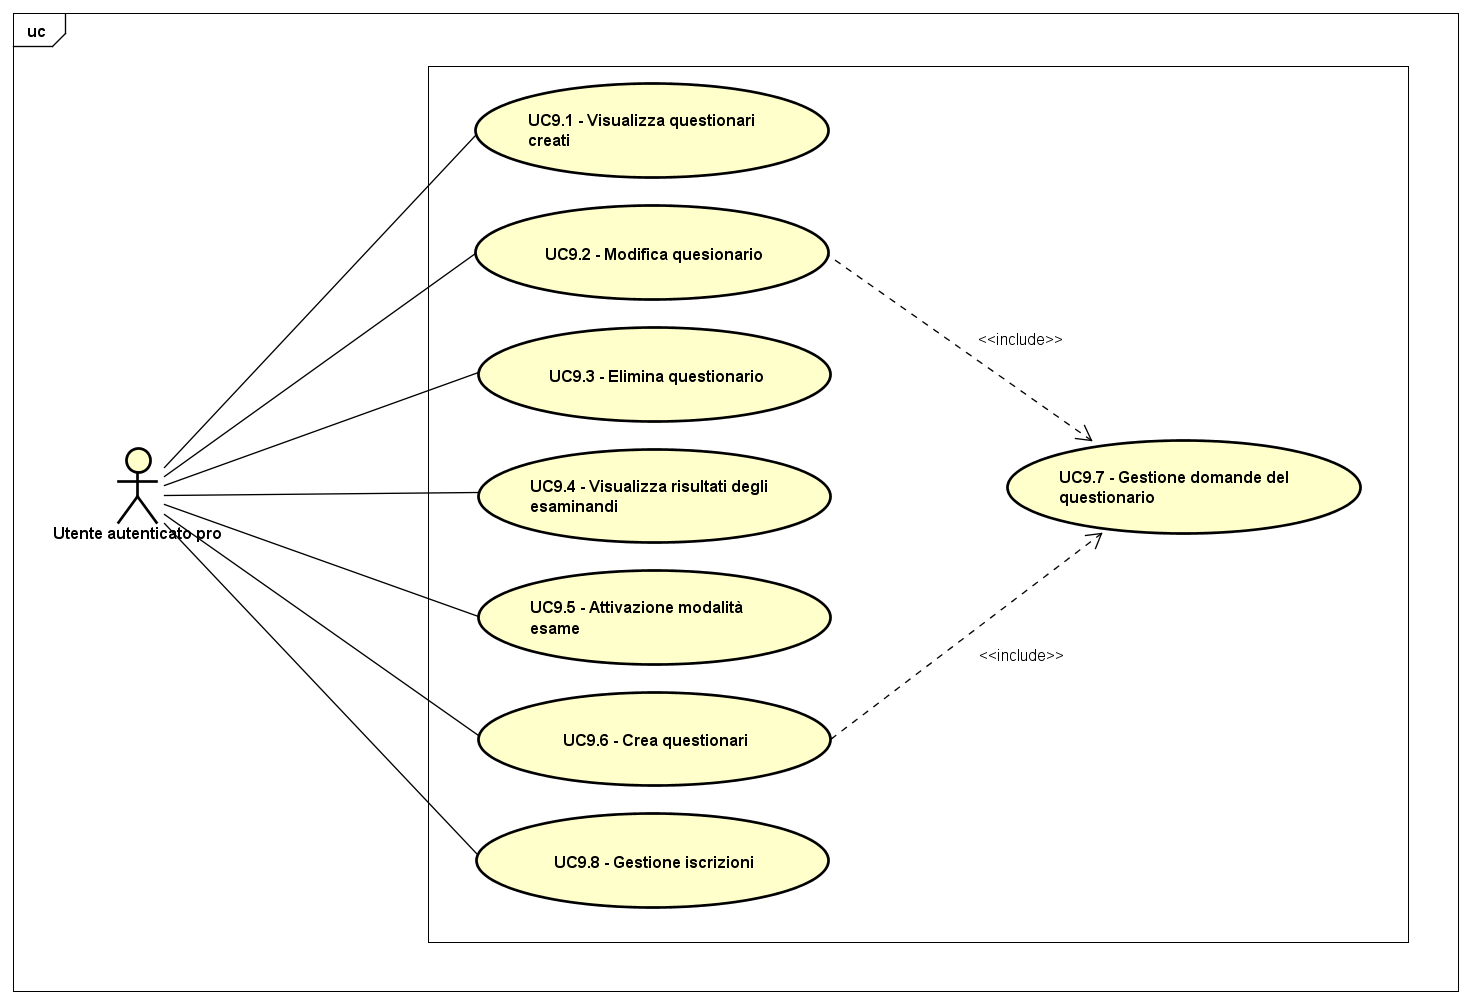
\includegraphics[scale=0.445,keepaspectratio]{UML/UC9.png}
	\caption{UC9: Gestione dei questionari}
\end{figure}
\FloatBarrier
\begin{itemize}
	\item \textbf{Attori}: \uaupro{};
	\item \textbf{Descrizione}: l'attore può modificare e/o eliminare i questionari creati da se stesso, crearne di nuovi, gestire le iscrizioni per i questionari ed infine attivare la modalità esame; 
	\item \textbf{Precondizione}: il sistema mostra la sezione della gestione dei questionari;
	\item \textbf{Postcondizione}: il sistema ha attuato le modifiche effettuate dall'attore ai propri questionari;
	\item \textbf{Scenario principale}:
		\begin{enumerate}
			\item L'attore può visualizzare i questionati creati (UC9.1);
			\item L'attore può modificare un questionario (UC9.2);
			\item L'attore può eliminare un questionario (UC9.3);
			\item L'attore può visualizzare i risultati degli esaminandi (UC9.4);
			\item L'attore può attivare la modalità esame di un questionario (UC9.5);
			\item L'attore può creare un questionario (UC9.6);
			\item L'attore può creare gestire le iscrizioni degli utenti per gli esami (UC9.8).
		\end{enumerate}
		\item \textbf{Inclusioni}: l'attore può gestire le domande di un questionario (UC9.7).		
\end{itemize}
							
	\subsubsection{Caso d'uso UC9.1: Visualizza questionari creati}
	\label{UC9.1}
	\begin{itemize}
		\item \textbf{Attori}: \uaupro{};
		\item \textbf{Descrizione}: l'attore può visualizzare i questionari da lui creati e selezionarne uno;
		\item \textbf{Precondizione}: il sistema mostra la possibilità di visualizzare i questionari creati;
		\item \textbf{Postcondizione}: l'attore visualizza i questionari da lui creato;
	\end{itemize}
	
	\subsubsection{Caso d'uso UC9.2: Modifica questionario}
	\label{UC9.2}
	\begin{figure}[h]
		\centering
	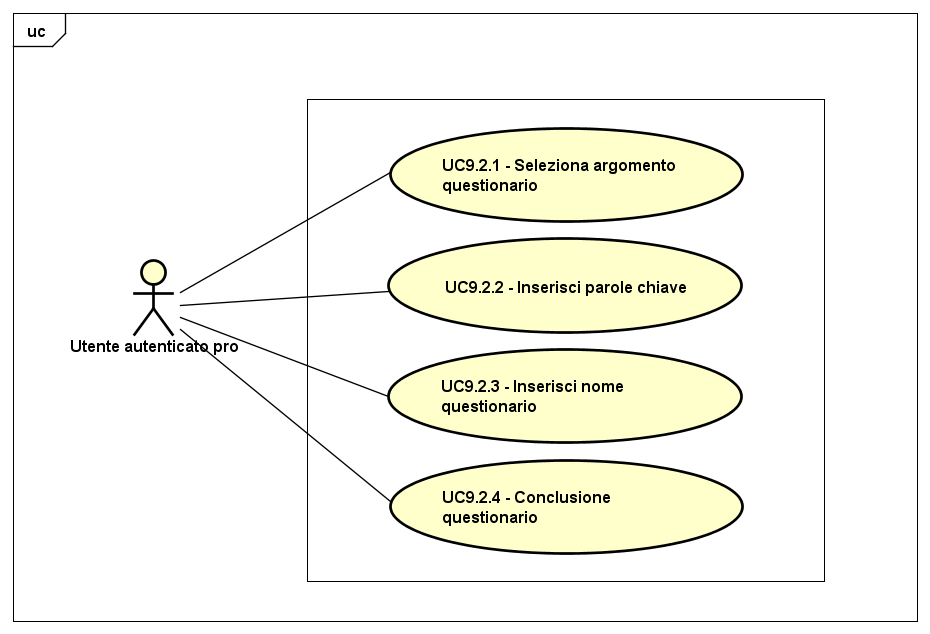
\includegraphics[scale=0.5,keepaspectratio]{UML/UC9_2.png}
		\caption{UC9.2: Modifica questionario}
	\end{figure}
	\FloatBarrier
	\begin{itemize}
		\item \textbf{Attori}: \uaupro{};
		\item \textbf{Descrizione}: l'attore può modificare il questionario selezionato;
		\item \textbf{Precondizione}: il sistema visualizza i questionari creati;
		\item \textbf{Postcondizione}: l'attore ha modificato il questionario selezionato; 
		\item \textbf{Scenario principale}:
			\begin{enumerate}
				\item L'attore può modificare il nome del questionario (UC9.2.1);
				\item L'attore può confermare le modifiche apportare (UC9.2.2).
			\end{enumerate}
	\end{itemize}
						
		\subsubsection{Caso d'uso UC9.2.1: Modifica nome questionario}
		\label{UC9.2.1}
		\begin{itemize}
			\item \textbf{Attori}: \uaupro{};
			\item \textbf{Descrizione}: l'attore può modificare il nome del questionario; 
			\item \textbf{Precondizione}: il sistema visualizza l'opzione di modifica nome questionario;
			\item \textbf{Postcondizione}: l'attore ha modificato il nome del questionario; 
			\item \textbf{Scenario principale}: l'attore modifica il nome del questionario.
		\end{itemize}
																		
		\subsubsection{Caso d'uso UC9.2.2: Conferma modifiche}
		\label{UC9.2.2}
		\begin{itemize}
			\item \textbf{Attori}: \uaupro{};
			\item \textbf{Descrizione}: l'attore può confermare le modifiche effettuate al questionario;
			\item \textbf{Precondizione}: il sistema visualizza l'opzione per confermare le modifiche effettuate;
			\item \textbf{Postcondizione}: l'attore ha confermato le modifiche effettuate;
			\item \textbf{Scenario principale}: l'attore conferma le modifiche effettuate;
			\item \textbf{Scenari alternativi}: l'attore non conferma e le modifiche fatte non vengono salvate. L'attore viene rimandato alla pagina contenente la lista dei questionari da lui creati.
		\end{itemize}
									
	\subsubsection{Caso d'uso UC9.3: Elimina questionario}
	\label{UC9.3}
	\begin{figure}[h]
		\centering
	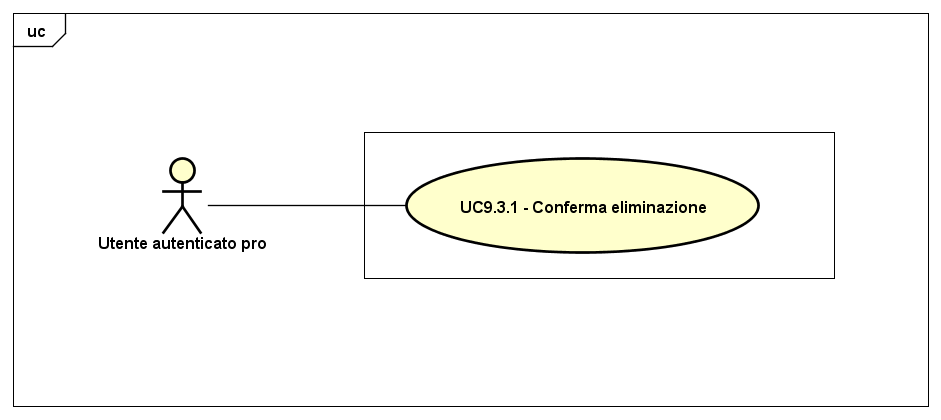
\includegraphics[scale=0.5,keepaspectratio]{UML/UC9_3.png}
		\caption{UC9.3: Elimina questionario}
	\end{figure}
	\FloatBarrier
	\begin{itemize}
		\item \textbf{Attori}: \uaupro{};
		\item \textbf{Descrizione}: l'attore può eliminare il questionario dall'archivio dei questionari;
		\item \textbf{Precondizione}: il sistema visualizza i questionari creati;
		\item \textbf{Postcondizione}: l'attore ha eliminato il questionario;
		\item \textbf{Scenario principale}: l'attore deve confermare di voler eliminare il questionario (UC9.3.1).
	\end{itemize}
	
		\subsubsection{Caso d'uso UC9.3.1: Conferma eliminazione}
		\label{UC9.3.1}
		\begin{itemize}
			\item \textbf{Attori}: \uaupro{};
			\item \textbf{Descrizione}: l'attore può confermare di voler eliminare il questionario; 
			\item \textbf{Precondizione}: il sistema visualizza l'opzione di conferma per l'eliminazione del questionario;
			\item \textbf{Postcondizione}: l'attore ha confermato di voler eliminare il questionario;
			\item \textbf{Scenario principale}: l'attore conferma di voler eliminare il questionario;
			\item \textbf{Scenari alternativi}: l'attore non conferma di voler eliminare il questionario. L'attore viene rimandato alla pagina contenente la lista dei questionari da lui creati.
		\end{itemize}
								
	\subsubsection{Caso d'uso UC9.4: Visualizza risultati degli esaminandi}
	\label{UC9.4}
	\begin{itemize}
		\item \textbf{Attori}: \uaupro{};
		\item \textbf{Descrizione}: l'attore può visualizzare le statistiche relative all'esito di un  questionario compilato dagli esaminandi;
		\item \textbf{Precondizione}: il sistema visualizza l'opzione per visualizzare i risultati degli esaminandi;
		\item \textbf{Postcondizione}: il sistema ha eseguito le opzioni scelte dall'attore;
		\item \textbf{Scenario principale}: l'attore visualizza le statistiche relative all'esito di un questionario compilato dagli esaminandi. 
	\end{itemize}
		
	\subsubsection{Caso d'uso UC9.5: Attivazione modalità esame}
	\label{UC9.5}
	\begin{itemize}
		\item \textbf{Attori}: \uaupro{};
		\item \textbf{Descrizione}: l'attore può attivare l'esame cosicché esso sia compilabile ai \uaus{};
		\item \textbf{Precondizione}: il sistema visualizza l'opzione per poter attivare la modalità esame su un determinato questionario;
		\item \textbf{Postcondizione}: il sistema ha attivato l'esame cosicché esso possa essere compilato dagli \uaus{} iscritti;
		\item \textbf{Scenario principale}: l'attore attiva l'esame cosicché esso possa essere compilato dagli \uaus{} iscritti.
	\end{itemize}
										
	\subsubsection{Caso d'uso UC9.6: Crea questionari}
	\label{UC9.6}
	\begin{figure}[h]
		\centering
	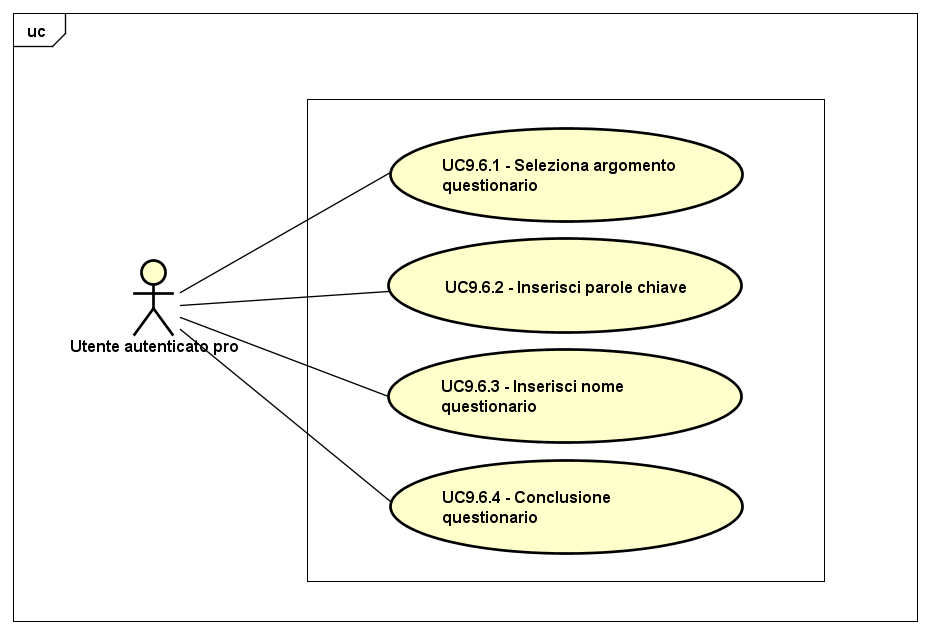
\includegraphics[scale=0.5,keepaspectratio]{UML/UC9_6.png}
		\caption{UC9.6: Crea questionari}
	\end{figure}
	\FloatBarrier
	\begin{itemize}
		\item \textbf{Attori}: \uaupro{};
		\item \textbf{Descrizione}: l'attore può creare un nuovo questionario; 
		\item \textbf{Precondizione}: il sistema visualizza l'opzione per creare nuovi questionari;
		\item \textbf{Postcondizione}: l'attore ha creato un questionario;
		\item \textbf{Scenario principale}:
			\begin{enumerate}
				\item L'attore può selezionare l'argomento del questionario (UC9.6.1);
				\item L'attore può inserire il nome del questionario (UC9.6.2);
				\item L'attore può selezionare gli argomenti del questionario (UC9.6.3);
				\item L'attore può concludere il questionario (UC9.6.4).
			\end{enumerate}
	\end{itemize}
	
		\subsubsection{Caso d'uso UC9.6.1: Seleziona argomento questionario}
		\label{UC9.6.1}
		\begin{itemize}
			\item \textbf{Attori}: \uaupro{};
			\item \textbf{Descrizione}: l'attore può selezionare l'argomento del questionario; 
			\item \textbf{Precondizione}: il sistema visualizza l'opzione per poter selezionare un argomento del questionario;
			\item \textbf{Postcondizione}: l'attore ha selezionato l'argomento del questionario;
			\item \textbf{Scenario principale}: l'attore seleziona l'argomento del questionario.
		\end{itemize}
		
		\subsubsection{Caso d'uso UC9.6.2: Inserisci parole chiave}
		\label{UC9.6.2}
		\begin{itemize}
			\item \textbf{Attori}: \uaupro{};
			\item \textbf{Descrizione}: l'attore può inserire delle parole chiave che identifichino il questionario; 
			\item \textbf{Precondizione}: il sistema visualizza l'opzione per poter inserire una parola chiave;
			\item \textbf{Postcondizione}: l'attore ha inserito delle parole chiave fino ad un massimo di quattro; 
			\item \textbf{Scenario principale}: l'attore inserisce le parole chiave che identificano il questionario.
		\end{itemize}
			
		\subsubsection{Caso d'uso UC9.6.3: Inserisci nome questionario}
		\label{UC9.6.3}
		\begin{itemize}
			\item \textbf{Attori}: \uaupro{};
			\item \textbf{Descrizione}: l'attore può inserire il nome del questionario; 
			\item \textbf{Precondizione}: il sistema visualizza l'opzione per poter inserire il nome del questionario;
			\item \textbf{Postcondizione}: l'attore ha inserito il nome del questionario; 
			\item \textbf{Scenario principale}: l'attore inserisce il nome del questionario.
		\end{itemize}
				
		\subsubsection{Caso d'uso UC9.6.4: Conclusione questionario}
		\label{UC9.6.4}
		\begin{figure}[h]
			\centering
			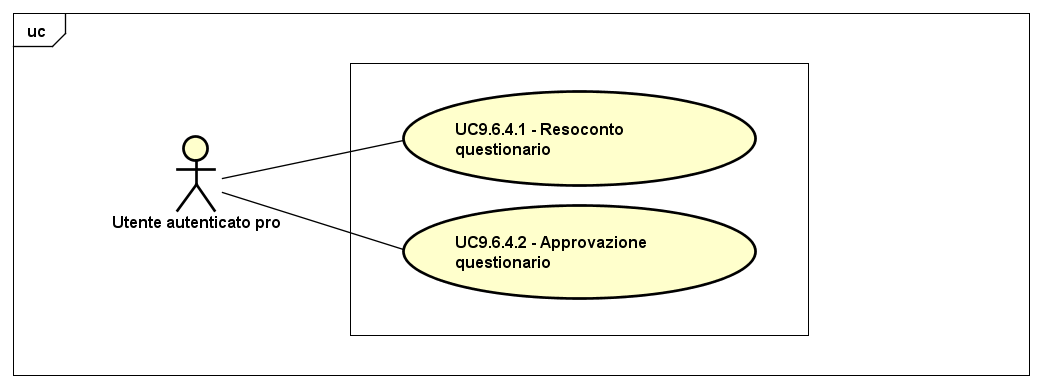
\includegraphics[scale=0.5,keepaspectratio]{UML/UC9_6_4.png}
			\caption{UC9.6.4: Conclusione questionario}
		\end{figure}
		\FloatBarrier
		\begin{itemize}
			\item \textbf{Attori}: \uaupro{}; 
			\item \textbf{Descrizione}: l'attore può smettere di inserire domande e concludere il questionario;
			\item \textbf{Precondizione}: il sistema visualizza l'opzione per poter concludere la creazione del questionario;
			\item \textbf{Postcondizione}: l'attore ha completato il questionario;
			\item \textbf{Scenario principale}: 
				\begin{enumerate}
					\item L'attore visualizza il riepilogo finale del questionario appena creato (UC9.6.4.1); 
					\item L'attore approva la creazione del questionario (UC9.6.4.2).
				\end{enumerate}
		\end{itemize}
				
			\subsubsection{Caso d'uso UC9.6.4.1: Resoconto questionario}
			\label{UC9.6.4.1}
			\begin{itemize}
				\item \textbf{Attori}: \uaupro{};
				\item \textbf{Descrizione}: l'attore può visualizzare le scelte fatte finora durante la creazione del questionario;
				\item \textbf{Precondizione}: il sistema visualizza il resoconto del questionario appena creato;
				\item \textbf{Postcondizione}: l'attore ha visualizzato le scelte fatte finora durante la creazione del questionario;
				\item \textbf{Scenario principale}: l'attore visualizza le scelte fatte finora durante la creazione del questionario.
			\end{itemize}
			
			\subsubsection{Caso d'uso UC9.6.4.2: Approvazione questionario}
			\label{UC9.6.4.2}
			\begin{itemize}
				\item \textbf{Attori}: \uaupro{};
				\item \textbf{Descrizione}: l'attore può approvare il questionario appena creato;
				\item \textbf{Precondizione}: il sistema visualizza l'opzione per poter approvare il questionario appena creato;
				\item \textbf{Postcondizione}: l'attore ha approvato il questionario;
				\item \textbf{Scenario principale}: l'attore approva il questionario;
				\item \textbf{Scenari alternativi}: l'attore non approva il questionario e quest'ultimo non viene archiviato. L'attore viene mandato alla pagina precedente.
			\end{itemize}				
	 
	 \subsubsection{Caso d'uso UC9.7: Gestione domande del questionario}
	 \label{UC9.7}
	 \begin{figure}[h]
	 	\centering
	 	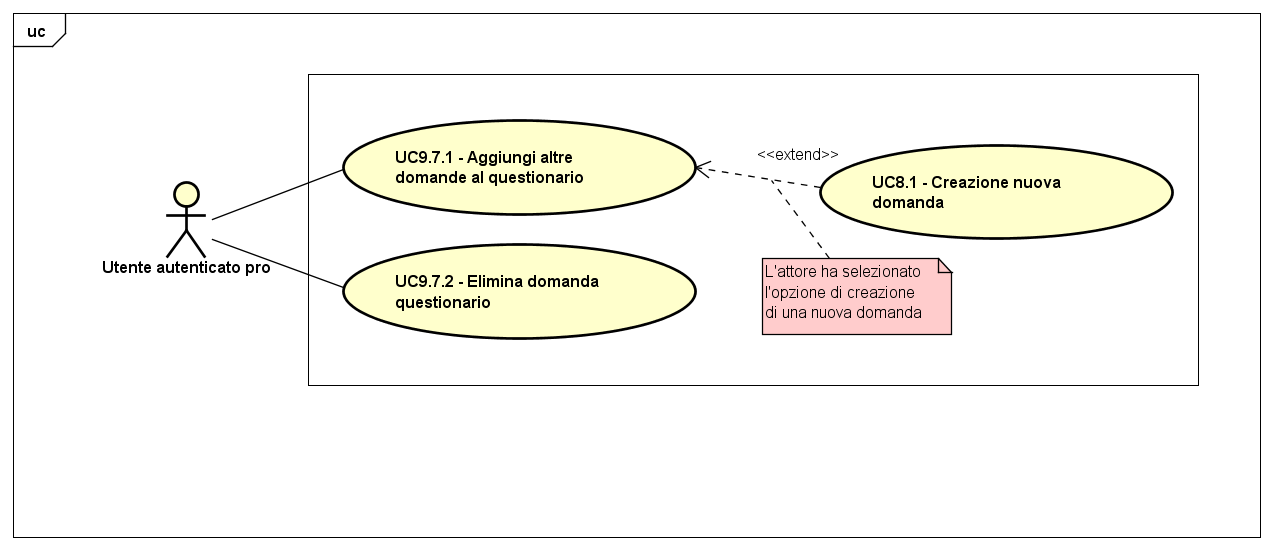
\includegraphics[scale=0.45,keepaspectratio]{UML/UC9_7.png}
	 	\caption{UC9.7: Gestione domande del questionario}
	 \end{figure}
	 \FloatBarrier
	 \begin{itemize}
	 	\item \textbf{Attori}: \uaupro{};
	 	\item \textbf{Descrizione}: l'attore può gestire le domande di un proprio questionario, aggiungendone oppure togliendone;
	 	\item \textbf{Precondizione}: il sistema visualizza l'opzione per la gestione delle domande nelle fasi di \\creazione/modifica di un questionario;
	 	\item \textbf{Postcondizione}: l'attore ha gestito le domande di un questionario;
	 	\item \textbf{Scenario principale}: 
	 	\begin{enumerate}
	 		\item L'attore aggiunge altre domande (UC9.7.1);
	 		\item L'attore elimina una domanda (UC9.7.2).
	 	\end{enumerate}
	 	\item \textbf{Estensioni}: l'attore può creare delle nuove domande per il questionario (UC8.1).		
	 \end{itemize}
	 
		 \subsubsection{Caso d'uso UC9.7.1: Aggiungi altre domande}
		 \label{UC9.7.1}
		 \begin{figure}[h]
		 	\centering
		 	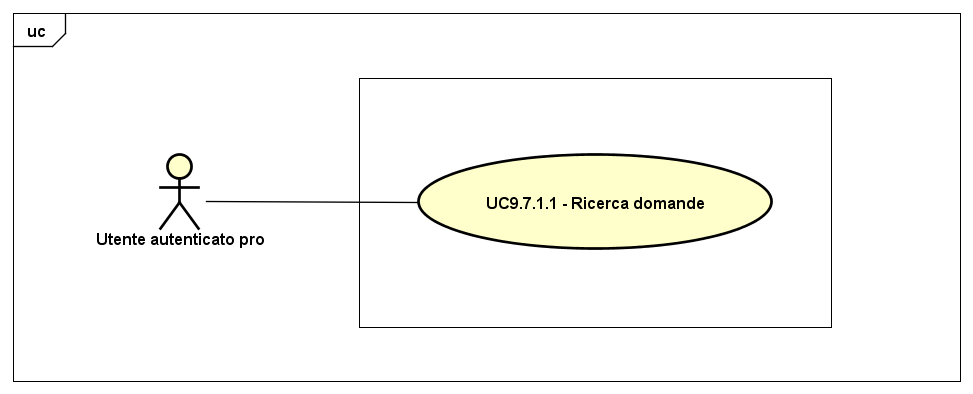
\includegraphics[scale=0.5,keepaspectratio]{UML/UC9_7_1.png}
		 	\caption{UC9.7.1: Aggiungi altre domande}
		 \end{figure}
		 \FloatBarrier
		 \begin{itemize}
		 	\item \textbf{Attori}: \uaupro{};
		 	\item \textbf{Descrizione}: l'attore può aggiungere altre domande cercando tra quelle già memorizzate nell'archivio oppure creandone una nuova; 
		 	\item \textbf{Precondizione}: il sistema visualizza l'opzione per poter aggiungere altre domande;
		 	\item \textbf{Postcondizione}: l'attore ha aggiunto nuove domande;
		 	\item \textbf{Scenario principale}: l'attore può eseguire una ricerca delle domande archiviate (UC9.7.1.1).
		 \end{itemize}
		 
			 \subsubsection{Caso d'uso UC9.7.1.1: Ricerca domande}
			 \label{UC9.7.1.1}
			 \begin{figure}[h]
			 	\centering
			 	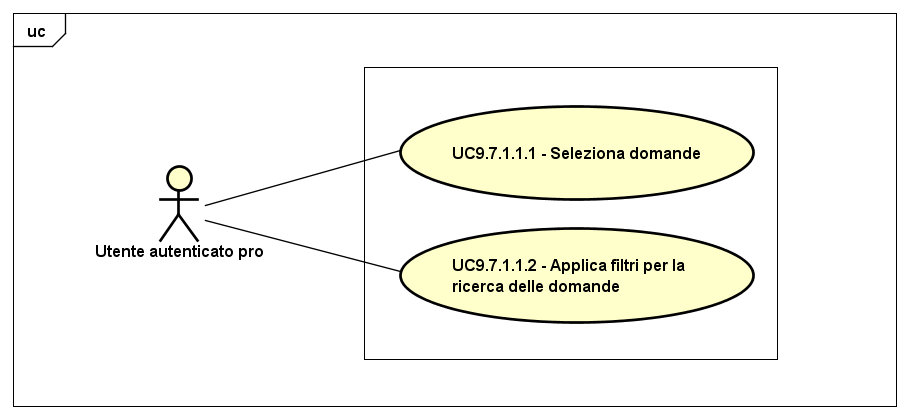
\includegraphics[scale=0.5,keepaspectratio]{UML/UC9_7_1_1.png}
			 	\caption{UC9.7.1.1: Ricerca domande}
			 \end{figure}
			 \FloatBarrier
			 \begin{itemize}
			 	\item \textbf{Attori}: \uaupro{};
			 	\item \textbf{Descrizione}: l'attore può eseguire una ricerca tra le domande archiviate; 
			 	\item \textbf{Precondizione}: il sistema visualizza l'opzione per ricercare le domande da inserire nel questionario;
			 	\item \textbf{Postcondizione}: l'attore ha ricercato tra le domande archiviate;
			 	\item \textbf{Scenario principale}:
			 	\begin{enumerate}
			 		\item L'attore può selezionare le domande (UC9.7.1.1.1); 
			 		\item L'attore può applicare dei filtri per la ricerca delle domande (UC9.7.1.1.2).
			 	\end{enumerate}
			 	\item \textbf{Estensioni}: nel caso in cui non ci sia nessun risultato dalla ricerca, all'attore viene proposta la possibilità di creare una nuova domanda (UC8.1).
			 \end{itemize}
			 
			 \subsubsection{Caso d'uso UC9.7.1.1.1: Seleziona domande}
			 \label{UC9.7.1.1.1}
			 \begin{itemize}
			 	\item \textbf{Attori}: \uaupro{};
			 	\item \textbf{Descrizione}: l'attore può selezionare le domande tra quelle ottenute dalla ricerca;
			 	\item \textbf{Precondizione}: il sistema visualizza l'opzione per poter selezionare una domanda da inserire nel questionario;
			 	\item \textbf{Postcondizione}: l'attore ha selezionato delle domande; 
			 	\item \textbf{Scenario principale}: l'attore seleziona le domande.
			 \end{itemize}
			 
			 \subsubsection{Caso d'uso UC9.7.1.1.2: Applica filtri per la ricerca delle domande}
			 \label{UC9.7.1.1.2}
			 \begin{itemize}
			 	\item \textbf{Attori}: \uaupro{};
			 	\item \textbf{Descrizione}: l'attore può applicare dei filtri per ottenere dei risultati migliori nelle ricerche: 
				 	\begin{itemize}
						\item Selezionare la difficoltà delle domande;
						\item Ordinarle per difficoltà;
						\item Ordinarle per parola chiave;
						\item Visualizzare quelle create da se stessi.
				 	\end{itemize}
			 	\item \textbf{Precondizione}: ;
			 	\item \textbf{Postcondizione}: il sistema visualizza l'opzione per poter applicare dei filtri alla ricerca; 
			 	\item \textbf{Scenario principale}: l'attore seleziona dei filtri da applicare per la ricerca.
			 \end{itemize}
		 
		 \subsubsection{Caso d'uso UC9.7.2: Elimina domanda dal questionario}
		 \label{UC9.7.2}
		 \begin{figure}[h]
		 	\centering
		 	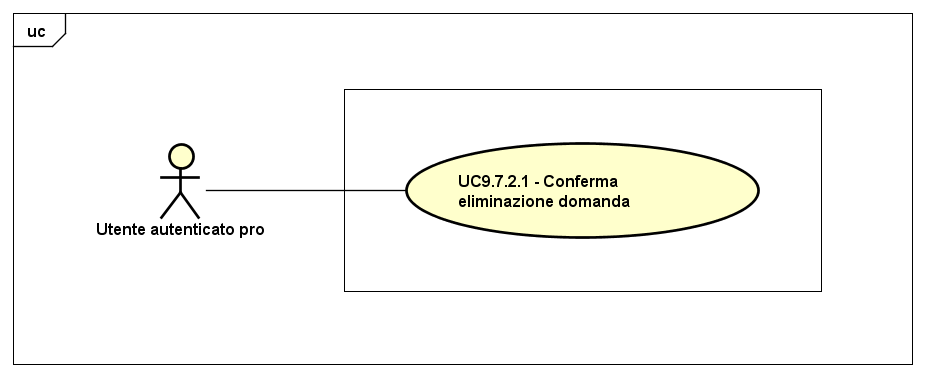
\includegraphics[scale=0.5,keepaspectratio]{UML/UC9_7_2.png}
		 	\caption{UC9.7.2: Elimina domanda dal questionario}
		 \end{figure}
		 \FloatBarrier
		 \begin{itemize}
		 	\item \textbf{Attori}: \uaupro{};
		 	\item \textbf{Descrizione}: l'attore può eliminare una domanda da un questionario;
		 	\item \textbf{Precondizione}: il sistema visualizza l'opzione per poter eliminare una domanda dal questionario;
		 	\item \textbf{Postcondizione}: l'attore ha eliminato una domanda;
		 	\item \textbf{Scenario principale}: l'attore può confermare di voler eliminare la domanda (UC9.7.2.1); 
		 	\item \textbf{Scenari alternativi}: l'attore ha cancellato tutte le domande. Deve allora inserirne almeno una, viene allora rimandato alla ricerca delle domande.
		 \end{itemize}
		 
		 \subsubsection{Caso d'uso UC9.7.2.1: Conferma eliminazione domanda}
		 \label{UC9.7.2.1}
		 \begin{itemize}
		 	\item \textbf{Attori}: \uaupro{};
		 	\item \textbf{Descrizione}: l'attore può confermare di voler eliminare la domanda;
		 	\item \textbf{Precondizione}: il sistema visualizza l'opzione per poter confermare l'eliminazione della domanda;
		 	\item \textbf{Postcondizione}: l'attore ha eliminato una domanda;
		 	\item \textbf{Scenario principale}: l'attore conferma di voler eliminare la domanda;
		 	\item \textbf{Scenari alternativi}: l'attore annulla l'eliminazione della domanda, viene allora rimandato alla schermata precedente.
		 \end{itemize}
		 
	 \subsubsection{Caso d'uso UC9.8: Gestione iscrizioni}
	 \label{UC9.8}
	 \begin{figure}[h]
	 	\centering
	 	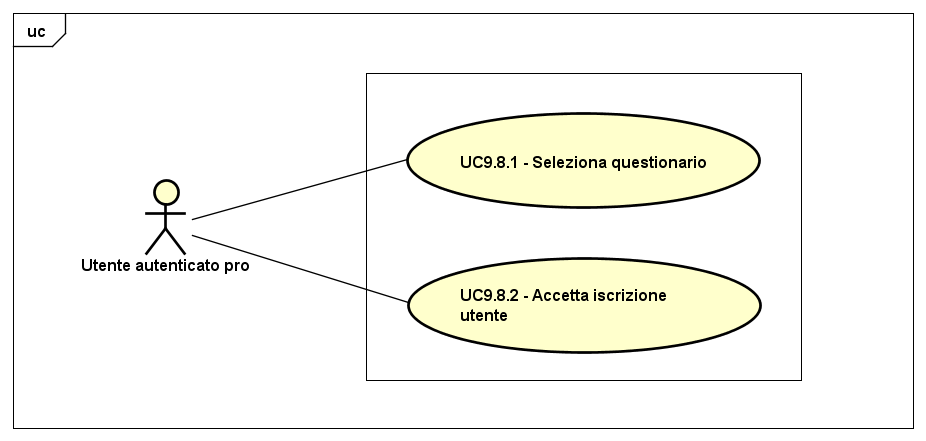
\includegraphics[scale=0.5,keepaspectratio]{UML/UC9_8.png}
	 	\caption{UC9.8: Gestione iscrizioni}
	 \end{figure}
	 \FloatBarrier
	 \begin{itemize}
	 	\item \textbf{Attori}: \uaupro{};
	 	\item \textbf{Descrizione}: l'attore può approvare le iscrizioni, per far in modo che gli utenti possano compilare un suo questionario;
	 	\item \textbf{Precondizione}: il sistema visualizza l'opzione per poter gestire le iscrizioni degli esaminandi ai questionari;
	 	\item \textbf{Postcondizione}: l'attore ha approvato la partecipazione degli utenti che vogliono prendere parte al questionario;
	 	\item \textbf{Scenario principale}: l'attore seleziona quale questionario gestire (UC9.8.1).
	 \end{itemize}
	 
		 \subsubsection{Caso d'uso UC9.8.1: Seleziona questionario}
		 \label{UC9.8.1}
		 \begin{itemize}
		 	\item \textbf{Attori}: \uaupro{};
		 	\item \textbf{Descrizione}: l'attore può selezionare il questionario del quale vuole approvare l'iscrizione degli utenti che vogliono prenderne parte. Di questo ne visualizzerà l'elenco degli utenti che hanno richiesto la partecipazione; 
		 	\item \textbf{Precondizione}: il sistema visualizza l'opzione per poter selezionare il questionario da gestire;
		 	\item \textbf{Postcondizione}: l'attore ha selezionato quale questionario gestire;
		 	\item \textbf{Scenario principale}: l'attore deve decidere quali utenti, tra quelli che vogliono partecipare, iscrivere al questionario (UC9.8.1.1).
		 \end{itemize}
		 
		 \subsubsection{Caso d'uso UC9.8.2: Accetta iscrizione utente}
		 \label{UC9.8.2}
		 \begin{itemize}
			 	\item \textbf{Attori}: \uaupro{};
			 	\item \textbf{Descrizione}: l'attore può decidere quali utenti accettare, tra quelli che vogliono partecipare al questionario; 
			 	\item \textbf{Precondizione}: il sistema visualizza il questionario selezionato dall'attore; 
			 	\item \textbf{Postcondizione}: l'attore ha approvato la partecipazione dell'\uau{} che richiede di iscriversi al questionario;
			 	\item \textbf{Scenario principale}: l'attore approva l'\uau{} che ha fatto richiesta per la partecipazione al questionario; 
			 	\item \textbf{Scenari alternativi}: nel caso in cui un \uau{} che vuole partecipare, non venga approvato, esso non avrà possibilità di accedere al questionario e ne sarà escluso.
		 \end{itemize}
			
				